

\chapter{Crisi della fisica classica}

\section{Corpo Nero}
	Idealmente un corpo nero rappresenta un oggetto che assorbe tutta l'energia della radiazione elettromagnetica incidente. \newline
In pratica potremo pensare ad esso come una cavit\`a (ad esempio sferica) su cui si trova un piccolo foro. se nel foro entra radiazione, questa verr\`a riflessa all'infinito al suo interno fino ad essere assorbita dalle pareti.

Trattando il problema classicamente, otteniamo che il potere emissivo della cavità sar\`a funzione di due fattori:

\begin{enumerate}
	\item la temperatura del sistema T
	\item la lunghezza d'onda della radiazione iniettata $\lambda $
\end{enumerate}	

ossia, in formule

\begin{equation}
\rho( \lambda, T) \sim \sigma T^4 \sim \frac{8\pi K_b T}{\lambda^4}
\end{equation}

Ma c'\`e un problema! Siccome in molti casi  $\lambda \to 0$, come per gli UV \newline ($10^{-8}$ m) e per i raggi $\gamma$ ($10^{-12}$ m),si avrebbe che 

\begin{equation}
\rho( \lambda, T)|_{T= cost.} \to \infty
\end{equation}

ossia avremmo la cosiddetta \textbf{catastrofe ultravioletta}.\newline
Questo ovviamente non succede, altrimenti il sole, essendo una fonte di UV, ci avrebbe gi\`a disintegrato da tempo.\newline
\newline
\newline
\noindent A questo punto entra in gioco \textbf{Planck}, chiedendosi: "sar\`a vero che la luce \`e un'onda? E se invece avesse una netta natura corpuscolare? E se la sua energia fosse discreta (o \textbf{quantizzata})?"

Il giovane genio Plack ipotizz\`o pertanto che la densit\`a di energia irradiata da un corpo nero fosse in realt\`a multiplo di un'energia quantizzata, ottenendo

\begin{equation}
\rho(\lambda. T) \sim \frac{8\pi h c}{\lambda^5} \frac{1}{e^{\frac{hc}{\lambda k T}} -1}
\end{equation}

Notiamo che espandendo in serie di Taylor questa converge.\\




\section{Effetto fotoelettrico}

Si nota quando, irradiando un metallo con onde elettromagnetiche, questo emette elettroni (un esempio pratico sono le scintille emesse durante la saldatura).

Venne scoperto da Hertz, il quale notò diversi fatti interessanti:

\begin{enumerate}

\item Il numero di elettroni emessi e la loro energia \textbf{non dipendono dall'intensit\`a della radiazione} (ossia dal numero di fotoni incidenti), ma \textbf{solamente dalla loro lunghezza d'onda $\lambda$.}

\item La quantità di corrente dipende invece dall'intensit\`a
\end{enumerate}

Tuttavia poteva ancora essere vera l'ipotesi ondulatoria della radiazione elettromagnetica, dato che \textbf{il fotone incide con una certa frequenza, viene assorbito da un'elettrone che oscilla come un dipolo e ne emette a sua volta uno con la stessa frequenza}. In realtà no.



\section{Effetto Compton}

Si tratta di scattering elastico dei fotoni incidenti sugli elettroni negli orbitali. Questo fenomeno cozza drammaticamente con la definizione ondulatoria della luce, dato che l'urto elastico è proprietà delle particelle. \newline
Compton scoprì che i fotoni scatterati avevano una diversa lunghezza d'onda rispetto a prima dell'urto, dipendente dall'angolo di impatto:

\begin{equation}
\Delta \lambda = \frac{h}{m_e c}(1 - cos(\theta))
\end{equation}

Elaboriamo meglio. Partiamo da due ipotesi:

\begin{enumerate}
	\item Il fotone viene solo assorbito
	\item L'angolo a cui viene emesso un fotone dopo l'assorbimento dipende solo da $\lambda$
\end{enumerate}

Quello che ci aspettiamo \`e di ritrovare su una lastra rivelatrice tutti i fotoni che faremo incidere sul bersaglio in un unico punto individuato da $\theta$.\newline
Sperimentalmente invece trovo che \textbf{il numero è diviso in $\theta$ e $\theta'$}. Allora se $\lambda \sim \theta$ avremo che $\lambda' \ne \lambda$. Questo però implica che tali fotoni sono stati deflessi e non assorbiti! 

 \begin{figure}[!htb]
	\center{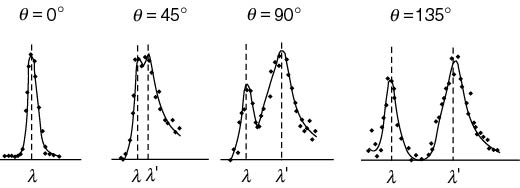
\includegraphics[width=\textwidth]
		{./images/4Idky.jpg}
	\caption{\label{fig:my-label} I = I($\lambda$)}}
\end{figure}

\section{Atomo di Bohr}

Lavorando sotto Rutherford, Bhor applicò l'ipotesi di Planck al suo modello atomico, enunciando tre postulati:

\begin{enumerate}
	
	\item Gli elettroni orbitano intorno al nucleo con orbite stabili (dette \textbf{stazionarie}) senza irraggiare. Possono muoversi da una all'altra ma non stare in mezzo.
	
	\item Le orbite stazionarie si trovano a distanze dal nucleo tali che il momento angolare orbitale degli elettroni sarà multiplo della costante di Plack ridotta.
	
	\begin{equation}
	|p_e|= m_e v r= n \hbar
	\end{equation}
	
	\item Gli elettroni possono spostarsi da un'orbita all'altra solo se ricevono o cedono un valore soglia di energia, detto \textbf{quanto}, pari a 
	
	\begin{equation}
	\Delta E = E_2 - E_1 = h \nu
	\end{equation}

\end{enumerate} 

\section{Figure d'Interferenza per fasci di elettroni}

Il fenomeno dell'interferenza si nota classicamente solo in caso di meccanica ondulatoria.
Per\`o se onsideriamo invece ora un fascio di elettroni con energia 

\begin{equation}
E= pc = \frac{hc}{\lambda}
\end{equation}

E lo facciamo incidere su una superficie con due fessure poste a distanza 

\begin{equation}
\vec{\lambda}= \frac{h}{\vec{p}}
\end{equation}

Se dietro tale superfice poniamo una lastra di materiale sensibile, noteremo la tipica figura d'interferenza... ma com'è possibile se l'elettrone è una particella?

Quanto detto fino ad ora ci porta a due conclusioni:

\begin{enumerate}
	\item La radiazione elettromagnetica e gli elettroni hanno una doppia natura, sia ondulatoria che corpuscolare
	\item L'energia di questi oggetti è quantizzata, ovvero che ciascuno di essi ha un'energia discreta e contribuisce a livello globale, ossia
	
	\begin{equation}
	E_{tot}= \sum{E_i} = h\sum{\nu_i}
\end{equation}

\end{enumerate}

Sappiamo, grazie alle nozioni di ottica, che l'intensità di un fascio di fotoni è data da

	\begin{equation}
	I = (E_1 + E_2)^2 = E_1^2 + E_2^2 + 2E_1E_2
\end{equation}

Questo significa, nel caso di singola particella che deve passare o da una fessura o dall'altra, che \textbf{il fotone interferisce con se stesso}. Gli elettroni si comportano allo stesso modo!

Dunque, se in \textbf{ottica classica} avevamo

\begin{equation}
\rho (r,t)= \rho_1 (r,t) + \rho_2 (r,t)
\end{equation}

In \textbf{meccanica quantistica} ci troveremo con

\begin{equation}
\psi (x,t)= \psi_1 (x,t) + \psi_2 (x,t)
\end{equation}

\begin{equation}
\psi_i (x,t)= A_i cos(kx-\omega t)
\end{equation}


 \begin{figure}[!htb]
	\begin{center}{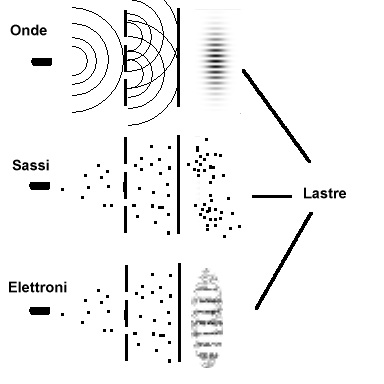
\includegraphics[width=.5\textwidth]
		{./images/Elettroni_e_fenditure.jpg}
		\caption{\label{fig:my-label} Rappresentazione del problema}}
	\end{center}
\end{figure}
